% THIS IS SIGPROC-SP.TEX - VERSION 3.1
% WORKS WITH V3.2SP OF ACM_PROC_ARTICLE-SP.CLS
% APRIL 2009
%
% It is an example file showing how to use the 'acm_proc_article-sp.cls' V3.2SP
% LaTeX2e document class file for Conference Proceedings submissions.
% ----------------------------------------------------------------------------------------------------------------
% This .tex file (and associated .cls V3.2SP) *DOES NOT* produce:
%       1) The Permission Statement
%       2) The Conference (location) Info information
%       3) The Copyright Line with ACM data
%       4) Page numbering
% ---------------------------------------------------------------------------------------------------------------
% It is an example which *does* use the .bib file (from which the .bbl file
% is produced).
% REMEMBER HOWEVER: After having produced the .bbl file,
% and prior to final submission,
% you need to 'insert'  your .bbl file into your source .tex file so as to provide
% ONE 'self-contained' source file.
%
% Questions regarding SIGS should be sent to
% Adrienne Griscti ---> griscti@acm.org
%
% Questions/suggestions regarding the guidelines, .tex and .cls files, etc. to
% Gerald Murray ---> murray@hq.acm.org
%
% For tracking purposes - this is V3.1SP - APRIL 2009
\usepackage(algorithm)
\usepackage(algorithmic)
\documentclass{acm_proc_article-sp}

\begin{document}

\title{Multipipes: Exploring Disjuntive Classifications in Hyperpipes}
\subtitle{[In an exciting manner]
\titlenote{A full version of this paper is available as
\textit{Author's Guide to Preparing ACM SIG Proceedings Using
\LaTeX$2_\epsilon$\ and BibTeX} at
\texttt{www.acm.org/eaddress.htm}}}

\numberofauthors{2} 
%
\author{
% The command \alignauthor (no curly braces needed) should
% precede each author name, affiliation/snail-mail address and
% e-mail address. Additionally, tag each line of
% affiliation/address with \affaddr, and tag the
% e-mail address with \email.
%
% 1st. author
\alignauthor
Aaron Riesbeck\\
       \affaddr{West Virginia University}\\
       \affaddr{100 Address Lane}\\
       \affaddr{Morgantown, WV 26505}\\
       \email{ariesbeck@theriac.org}
% 2nd. author
\alignauthor
Adam Brady\\
       \affaddr{West Virginia University}\\
       \affaddr{100 Fake St.}\\
       \affaddr{Morgantown, WV 26505}\\
       \email{adam.m.brady@gmail.com}
}
\date{12 October 2009}

\maketitle
\begin{abstract}

This paper explores classifiction with disjunctive sets using a modified form of HyperPipes called MultiPipes. Rather than apply HyperPipes it's intended sparse datasets, we find that it's application to non-sparse, many-class datasets typically results in several tied classification scores which we then union into a disjunction. This union presents interesting possibilities in it's high accuracy in containing the target class. Although we initially cannot predict single classes, we find that these disjunctions often eliminate large portions of possible classes. Essentialy we aren't certain what the class is, but we are very certain of what the class is not. The rest of the paper explores two alternative strategies with MultiPipes. The first involves methods of reducing the disjunctive sets to single classifications. The second considers growing the disjunctive sets to optimize the accuracy of containment vs. set size.

\end{abstract}

\keywords{HyperPipes, disjoint sets, \LaTeX, multiple classes, indecisive learners} % NOT required for Proceedings


\section{Introduction to HyperPipes}

HyperPipes is a learner originally offered by Eisenstein et al~\cite{Eisenstein04} for extremely large, sparse datasets. Rather than maintain a large working memory of statistics on each row of data, HyperPipes maintains a small data structure for each class that merely "remembers" whether a particular attribute has been encountered before. For numerics, a range of maximum and minimum values encountered is kept. When classifying, original HyperPipes classifies a row based on which class most "contains" the current attributes. For numeric attributes, a new instance is "contained" if it falls within the maximum and minimum values see so far.

This is perfect for sparse datsets, as your working memory need only contain one HyperPipe for each possible class, and each pipe must maintain only a the unique symbols encountered so far along with two numeric bounds for each column. The result is a fast, dumb, scalable learner.

One caveat remains in the HyperPipes algorithm. For large, sparse datasets there are enough unique columns to promote a wide variance in which HyperPipe best "contains" a class. However, for more traditional datasets with fewer columns HyperPipes' accuracy breaks down. By nature HyperPipes is strongly succeptible to outlier data, as the frequency of an encountered attribute is ignored and extremely high or low numerics will stretch the bounds. In this paper we explore a means to maintain the speed and scalability of HyperPipes while extending it's application to a wider variety of datasets.


\subsection{Pseudocode for hyperpipes}

%\begin{figure}
\begin{program}
%\footnotesize
\begin{algorithmic}
\Procedure {RunHyperPipes}{$Nothing$}
\State $HyperPipes := array[]$
\State $Guessed := 0$
\State $GuessedCorrect := 0$
\ForAll {$Line in DataFile$}
\State $Guessed++$
\State $GuessedCorrect \mbox{+=} Classify(MyHyperPipes,Line)$
\State $HyperPipes := AddExperience(Line,HyperPipes)$
\EndFor
\State $Accuracy := GuessedCorrect/Guessed$
\EndProcedure
\end{algorithmic}
\caption{HyperPipes Pseudo Code.}\label{Pseudocode}
\end{program}
%\end{figure}


\begin{program}
\begin{algorithmic}
\Procedure {Classify}{$HyperPipes$,$Line$}
\State{$BestScore := 0$}
\State{$BestClass := []$}
\ForAll{HPipe in HyperPipes}
\State{$HPipeScore := 0$}
\ForAll{Attr in Line}
\If{$Attr <= HPipe.Attr.max\; \&\&\; Attr >= HPipe.Attr.min$}
\State{$HPipeScore++$}
\EndIf
\EndFor
\If{$HPipeScore >= BestScore$}
\If{$HPipeScore := BestScore$}
\State{$BestClass := BestClass + HPipe.class$}
\Else
\State{$BestClass := array(HPipe.class)$}
\State{$BestScore := HPipeScore$}
\EndIf
\EndIf
\EndFor
\If{$BestClass\; contains\; Line.class$}
\State \Return 1
\EndIf
\State \Return 0
\EndProcedure
\end{algorithmic}
\caption{HyperPipes Classify Pseudo Code.}\label{PseudocodeClass}
\end{program}

\begin{program}
\begin{algorithmic}
\Procedure {AddExperience}{$HyperPipes$,$Line$}
\State{$CurrentPipe := FindPipe(Line.class,HyperPipes)$}
\If{$null\; CurrentPipe$}
\State{$HyperPipes := HyperPipes + CreateHyperPipe(Line.class)$}
\State{$CurrentPipe := FindPipe(Line.class,HyperPipes)$}
\EndIf
\ForAll{Attr in Line}
\State{$CurrentPipe.max := max(CurrentPipe.max,Attr)$}
\State{$CurrentPipe.min := min(CurrentPipe.min,Attr)$}
\EndFor
\EndProcedure
\end{algorithmic}
\caption{HyperPipes Classify Pseudo Code.}\label{PseudocodeClass}
\end{program}



\subsection{The Problem with HyperPipes}

\SubSubSection{Tied Classes}
During development of the original HyperPipes implementation it was noted 
that the code only kept track of the most recently seen class with a score 
equal to or greater than the largest score seen to that point. This means
that when running HyperPipes if multiple classes tied in score the class
tested last would be blindly chosen. We found that this anomoly caused our 
HyperPipes implementation to prefer the last classes discovered once it 
learns many rows.
\SubSubSection{Susceptible to Over Fitting}
HyperPipes has the ability to have very low overhead costs in terms of 
memory. However, this benefit is overshadowed by HyperPipes susceptibility 
to overfitting. As more and more rows are added as experience to a HyperPipe 
its min and max values with slowly approach the min and max of the attribute 
alone regardless of class. This causes HyperPipes guessing ability to 
completely fall apart. As the min and max values for the attributes in every
HyperPipe expand the scores become very high and the likelyhood of 
encountering the issue in the previous sub-section becomes greater. That is, 
as each of the HyperPipes expand their min and max attribute values start to 
become so similar to eachother that they all begin to acheive common scores.
\SubSubSection{Outliers Ruin Scoring}
As shown in the AddExperience function pseudocode a HyperPipe contains a set 
of bounds for each attribute. These bounds indicate the min and a max value 
ever seen for this attribute for this class. This becomes a problem when an 
outlier for that attribute occurs. Imagine after 10,000 rows your min is 23 
and your max is 45. You encounter a new row where this attributes value is 
431. This causes your new max value to be 431. This can be a major pitfall 
if this is the only time a number this large is encountered for this class. 
 You have now expanded this HyperPipe to a max so large that this attribute 
loses its ability to classify (It always matched on this attribute for this 
class).
\SubSubSection{Memory Management}
The original HyperPipes required prior knowledge of the dataset. In other 
words it created all of the necessary HyperPipes at the beginning and 
modified them as it went through the dataset. This means that if a new class 
is created the entire algorithm would have to start from the beginning with 
this knowledge that this new class existed. If you were able to control the
outliers and the over fitting for this algorithm you could use this type of 
classifier in a real world situation where ne classes are constantly being 
discovered. 

\subsection{Patching HyperPipes}

\subsubsection{Fixing Tied Classes}
When it was discovered that HyperPipes tended to choose classes 
towards the end of the classes list we investigated further to 
find that many classes were tieing against other classes. We 
then decided that this was unacceptable. Overwriting a class 
with another class of the same score puts a large emphasis on 
the order in which you score the classes. For this issue we 
decided to temporarily throw away the idea of classification 
and modified the code to return any classes who tied. This 
simple modification proved to us that this issue alone was a 
major factor in HyperPipes demise when put up against other 
classifiers. To recap the original hyperpipes said that if 
the current score is equal to or greater than the best score 
set the best class to the current class. After modification 
hyperpipes now states that if the score is greater than the 
best score set the best class to an array containing only the 
current class. If the current score is equal to the best score 
then append the current class to the list of best classes.
\subsubsection{Fixing Over Fitting}
As described previously Hyperpipes has an over fitting issue 
when it learns too much. While we have no implemented these 
potential fixes our possible solutions are described below:
\begin{itemize}
	\item{Limit Number of Rows To Be Learned}
	It might be effective to simply limit the number of rows 
	that HyperPipes will use when doing its learning. This 
	number of rows might be calculated based on the number 
	classes and it may also require that this limit be 
	evenly distributed across all classes.
	\item{Detect Overfitting by Class Overlap}
	It may be possible to detect over-fitting by determining 
	the amount of overlap between classes. In other words, 
	if the number of attributes in a HyperPipe reaches a 
	certain level we could say that we should not modify our 
	HyperPipes with the information learned in this new line
	as it would cause too much overlap between classes.
	\item{weighted distance}
	\item{centroids via overlap}
	\item{increasing alpha}
\end{itemize}
\subsubsection{Fixing Outliers}
\subsubsection{Fixing Memory Management}


\section{Narrowing vs. Classifying}

Why narrow when you can classify?


\section{Preliminary Results}

Description of results
\begin{itemize}
	\item{incremental learning}
	\item{batch learning}
	\item{weighted distance}
	\item{centroids via overlap}
	\item{increasing alpha}
\end{itemize}

\subsection{Disjoint Learning}

\begin{figure*}
\centering
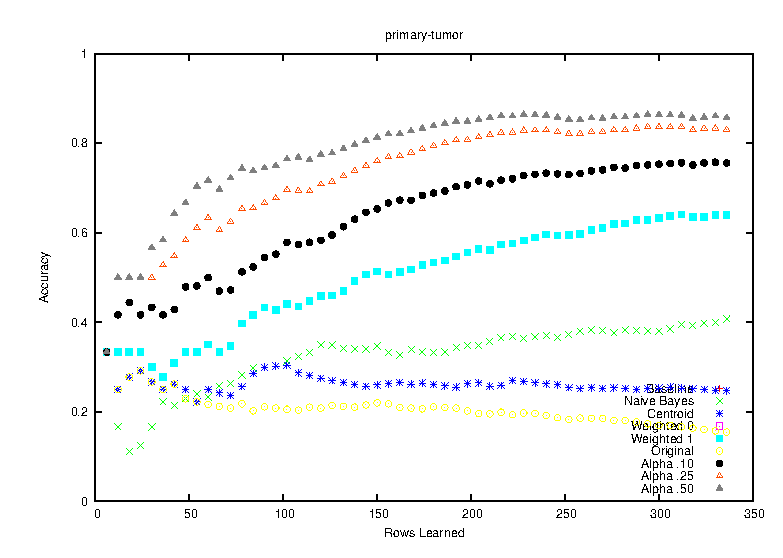
\epsfig{file=charts/primary-tumor.eps}
\caption{Incremental results from a discrete dataset with many class values.}
\label{fig:primary-tumor}
\end{figure*}

Learning with disjoint sets introduces some caveats to data analysis. As seen in ~\ref{fig:primary-tumor}, our baseline disjunctive HyperPipes consistently outperforms both naive bayes and the original HyperPipes algorithm. However, our disjuntive learner doesn't exactly play fair, hedgings it's bets with multiple predicted classes. Note as well that when we use our centroid method for single classification, we fail to consistently beat naive bayes.

However, when disjunctive HyperPipes cheats, it does so with a conscious. While the size of the disjunctions varies, on average the set contains only 4 out of 22 possible classes, or about 18\% of the original possible classes. As a result, we trade in single classification for a doubling of accuracy.


\subsection{Breaking the Ties}

While we believe the mutliple class result of HyperPipes is 
an interesting discovery we understand the need for a complete 
classification system. We have come up with two methods for
attempting to classify the result of MultiPipes into a single 
class and have come up with two different approaches. One 
approach was discovered when attempting to relieve outliers.
\subsubsection{Weighted Distance from Mean}
There are two methods we use for calculating the distance from 
the mean in our algorithm. As stated above in "Fixing Outliers" 
we noted that an attribute range scores a 1 if it falls within 
the min and max for that attribute in a class. Our modification, 
as stated above was to use a normalized calculation to determine 
a value between 0 and 1 based on the attribute values distance 
from the mean attribute value in that class. Two calculations 
were discussed and they are as follows:
\begin{enumerate}
\item Weighted Distance From Mean 1: In this calculation it was 
decided that the distance from mean should be calculated as:
\begin{equation}
  WghtDist=\frac{(Max-Min)-|(Mean-Val)|}{(Max-Min)}
\end{equation}
where Max, Min, and Mean are the max, min, and mean values for 
the attribute in the HyperPipe for the class currenlty being 
scored and Val is the current attribute value in the row being 
classified. 
\item Weighted Distance From Mean 2: The calculation in this 
method is slightly different from the one above:
\begin{equation}
  BigGap = max((Max-Mean),(Mean-Min))
\end{equation}
\begin{equation}
  WghtDist=\frac{(BigGap)-|(Mean-Val)|}{(BigGap)}
\end{equation}
where Max, Min, and Mean are the max, min, and mean values for 
the attribute in the HyperPipe for the class currenlty being 
scored and Val is the current attribute value in the row being 
classified.
\end{enumerate}



graph of weighted distance classification accuracy


Description of centroid acquisition from overlap

graph of centroid learning results



\subsection{Casting a wider net}

Description of alpha value

Purpose of alpha value for expanding class set

Results of expanding alpha (graph)

Analysis of growth in enclosure with alpha changes



\section{Preliminary Conclusions}

WE CONCLUDE


% The following two commands are all you need in the
% initial runs of your .tex file to
% produce the bibliography for the citations in your paper.
\bibliographystyle{abbrv}
\bibliography{multipipes}  %the name of the Bibliography in this case
% You must have a proper ".bib" file
%  and remember to run:
% latex bibtex latex latex
% to resolve all references

\subsection{References}
Generated by bibtex from your ~.bib file.  Run latex,
then bibtex, then latex twice (to resolve references)
to create the ~.bbl file.  Insert that ~.bbl file into
the .tex source file and comment out
the command \texttt{{\char'134}thebibliography}.
\balancecolumns
\end{document}
